\documentclass[diss-proposta,nocipinfo]{texufpel}
%nocipinfo para não aparecer os dados da CIP no Resumo

\usepackage[utf8]{inputenc} % acentuacao
\usepackage{graphicx} % para inserir figuras
\usepackage[T1]{fontenc}

\hypersetup{
    hidelinks, % Remove coloração e caixas
    unicode=true,   %Permite acentuação no bookmark
    linktoc=all %Habilita link no nome e página do sumário
}

\unidade{Centro de Desenvolvimento Tecnológico}
\programa{Programa de Pós-Graduação em Computação}
\curso{Ciência da Computação}

\title{Aplicação de Técnicas de Mineração de Dados e Learning Analytics para Predição de Evasão de Alunos na UFPel}

\author{Costa}{Alexandre Gomes da}
\advisor[Prof.~Dr.]{Mattos}{Julio Carlos Balzano de}
\coadvisor[Prof.~Dr.]{Primo}{Tiago Thompsen}

%Palavras-chave em PT_BR
\keyword{mineração de dados educacionais}
\keyword{learning analytics}
\keyword{técnicas de predição}
\keyword{kdd}
\keyword{descoberta de conhecimento em base de dados}

%Palavras-chave em EN_US
\keywordeng{educational data mining}
\keywordeng{learning analytics}
\keywordeng{prediction techniques}
\keywordeng{kdd}
\keywordeng{knowledge-discovery in databases}


\begin{document}

\maketitle 
\sloppy

%Resumo em Portugues (no maximo 1 pagina)
\begin{abstract}
Os sistemas de gestão para educação armazenam uma grande quantidade de dados oriundos de diversas modalidades de iteração entre alunos e professores mas também entre os alunos e o ambiente educacional (biblioteca, restaurantes universitários entre outros). Por exemplo, dados como notas, registro de presença de aluno, acesso ao sistema de biblioteca, logs de iteração com o sistema e vários outros tipos de atributos são ricos para a compreensão e auxílio nos processos de tomada de decisão em ambientes educacionais. Analisar e encontrar padrões nesta quantidade de dados manualmente é inviável humana e economicamente, por isso a utilização de Mineração de Dados Educacionais (MDE) e \textit{Learning Analytics (LA)} ganharam popularidade nos últimos anos. Este trabalho pretende explorar a utilização destas técnicas para extrair os dados do Sistema Integrado de Gestão da UFPel (Cobalto) visando criar modelos que levem a predição de alunos em risco de evasão para suporte aos processos de tomada de decisão na Universidade Federal de Pelotas. 

% Com o surgimento de sistemas de gestão da educação uma grande quantidade de dados vem sendo produzida através de diversas modalidade de iteração entre alunos e professores. Analisar essa quantidade de dados não é uma tarefa viável para o homem, por isso surge a Mineração de Dados Educacionais (MDE) e Learning Analytics (LA). Nos últimos anos, uma gama cada vez maior de trabalhos vem surgindo nas áreas de MDE e LA. Este trabalho será focado em extrair os dados do Sistema Integrado de Gestão da UFPel (Cobalto) para prever alunos em risco de evasão. A partir da aquisição dos dados serão aplicado técnicas de MDE e LA para chegar a um modelo de predição.


% Devido a essa grande quantidade de trabalhos é que se faz necessário fazer um levantamento para descobrir quais métodos, técnicas e algoritmos vem sendo utilizado, e ainda quais tipos de problemas vem sendo apurados. A pesquisa foi realizada, procurando responder as seguintes questões: Qual tem sido as técnicas utilizadas nos trabalhos na área. Qual tipo de dados estão sendo considerados pertinentes na área. Qual é o objetivo de estudo dos trabalhos na área. Qual são as ferramentas que tem sido utilizadas na área. O objetivo deste trabalho é fazer uma busca nas principais meios de publicações brasileiros que vem pesquisando MDE utilizando técnicas de predição.
\end{abstract}

\chapter{Motivação}
% (ENTRE 1 e 2 PÁGINAS)

% Nesta seção, apresenta-se um breve histórico da área de concentração
% da Dissertação, partindo do tema mais abrangente até chegar
% especificamente no assunto do Projeto. Além disso, apresenta-se a
% justificativa para a realização do trabalho, sua importância acadêmica
% ou para comunidade e grau de inovação. Poderá também apresentar as
% distinções entre o trabalho atual e outros trabalhos já realizados.

% *** Motivação: dados evasão do INEP, motivar o trabalho (já está) e colocar os trabalhos relacionados (para embasar o trabalho)
% Sequencia: evasão, etc -> TICs - TICs na evasão -> objetivo (teu trabalho)
% 1. Crescimento da Educação Superior
% 2. Taxas evasão, trancamento elevadas
% 3. Isto é um problema !
% 4. TICs
% 5. TICs no ambiente educacional (evasão)

% *** Metodologia

% Comparando os índices da Universidade Federal de Pelotas (UFPel) com os do \citet{inep:2018} estes índices não mudam muito. Em 2017 o índice de matriculas desvinculadas na UFPel foi de de 11,53\% que está abaixo do índice de 11,56\% apresentado pelo \citet{inep:2018}. Mas olhando para a evasão curso a curso no ano de 2017 observamos dados alarmantes. Por exemplo, temos cursos como o de Geoprocessamento onde a taxa de evasão foi de 29,07\%. Por isso esses dados mostram que a evasão também é um problema na UFPel e deve ser observada.

O uso constante de Tecnologia da Informação e Comunicação em diversas áreas vêm gerando um grande volume de dados. Tecnologias como a internet, redes sociais, ambientes virtuais de aprendizagem, dispositivo móveis, aplicativos embarcados, leitores de código de barras, sensores, leitores biométricos e sistemas de informação em geral são alguns exemplos de recursos que vem aumentando o número de dados das mais diversas naturezas \cite{goldschmidt2015data}.

%% Educação
Atualmente, as áreas como a educação produzem uma grande quantidade de dados relacionados a alunos e professores todos os dias. Para isto, esta área utiliza sistemas para fazer o controle de iterações acadêmicas, gestão de projetos de pesquisa, ensino ou extensão, ou até mesmo sistemas para fazer o controle de gestão de pessoas são alguns do exemplos de sistemas que podem gerar um volume considerável de dados com frequência.

A partir desse volume de dados é possível analisar problemas recorrentes relacionados a educação. Um desses problemas é a evasão escolar que ainda é um desafio a ser superado.
A evasão é um problema que atinge não só as Instituições de Ensino Superior (IES) privadas, mas também as públicas. Segundo dados do \citet{inep:2018}, em 2017, o índice de matrículas desvinculadas em todo o Brasil foi de 16,41\%. Já para as IES públicas esse índice no mesmo período foi de 11,56\%. Outro valor a ser considerado é o número de matriculas trancadas, onde foi de 11,17\% em todo o Brasil e 8,10\% IES públicas.

Comparando os índices da Universidade Federal de Pelotas (UFPel) com os do \citet{inep:2018} estes índices não mudam muito. Em 2017 o índice de matriculas desvinculadas na UFPel foi de de 11,53\% que está abaixo do índice de 11,56\% apresentado pelo \citet{inep:2018}. Mas olhando para a evasão curso a curso no ano de 2017 observamos dados alarmantes. Por exemplo, temos cursos como o de Geoprocessamento onde a taxa de evasão foi de 29,07\%.  Esse fenômeno é conhecido na estatística como paradoxo de Simpson, uma tendência aparece em um determinado grupo de dados e desaparece quando estes dados são combinado. Ou seja, olhando para os cursos individualmente vários deles apresentam uma taxa de evasão bem elevada, mas quando essas taxas são combinadas a taxa de evasão não é tão relevante \cite{wagner1982simpson}. Olhando para esses dados algumas perguntas surgem tais como "Qual é o perfil do aluno que tende a evadir?" ou "Qual é a quantidade de alunos que trancaram e acabaram evadindo?", por exempo.

%% Knowledge Discovery in Database - KDD
Embora com ajuda de ferramentas computacionais, analisar essa crescente quantidade de dados não é trabalho para o homem \cite{goldschmidt2015data}. Para ajudar nesta questão a área de Descoberta de Conhecimento em Base de Dados (\textit{Knowledge Discovery in Database} - KDD) é focada em extrair conhecimento encima de granes volumes de dados. O termo mais conhecido relacionado a essa área é a Mineração de Dados (MD) que é uma das etapas do processo de KDD.

%% Mineração de dados educacionais
Segundo \citet{Koedinger2008} Mineração de Dados (MD) aplicada à educação é um campo interdisciplinar emergente mais conhecido como Mineração de Dados Educacionais (MDE).
\citet{baker2010data} define MDE como a área de investigação científica centrada no desenvolvimento de métodos para fazer descobertas dentro dos tipos de dados que vêm de ambientes educacionais e usando esses métodos para entender melhor os alunos e a aprendizagem deles. A Figura \ref{fig:areas-relacionadas-mde} mostra que a área de MDE pode ser a combinação de 3 grandes áreas (ciência da computação, estatistia e educação) e serve de exemplo para justificar a interdisciplinaridade da área.

\begin{figure}[htbp]
  \centering 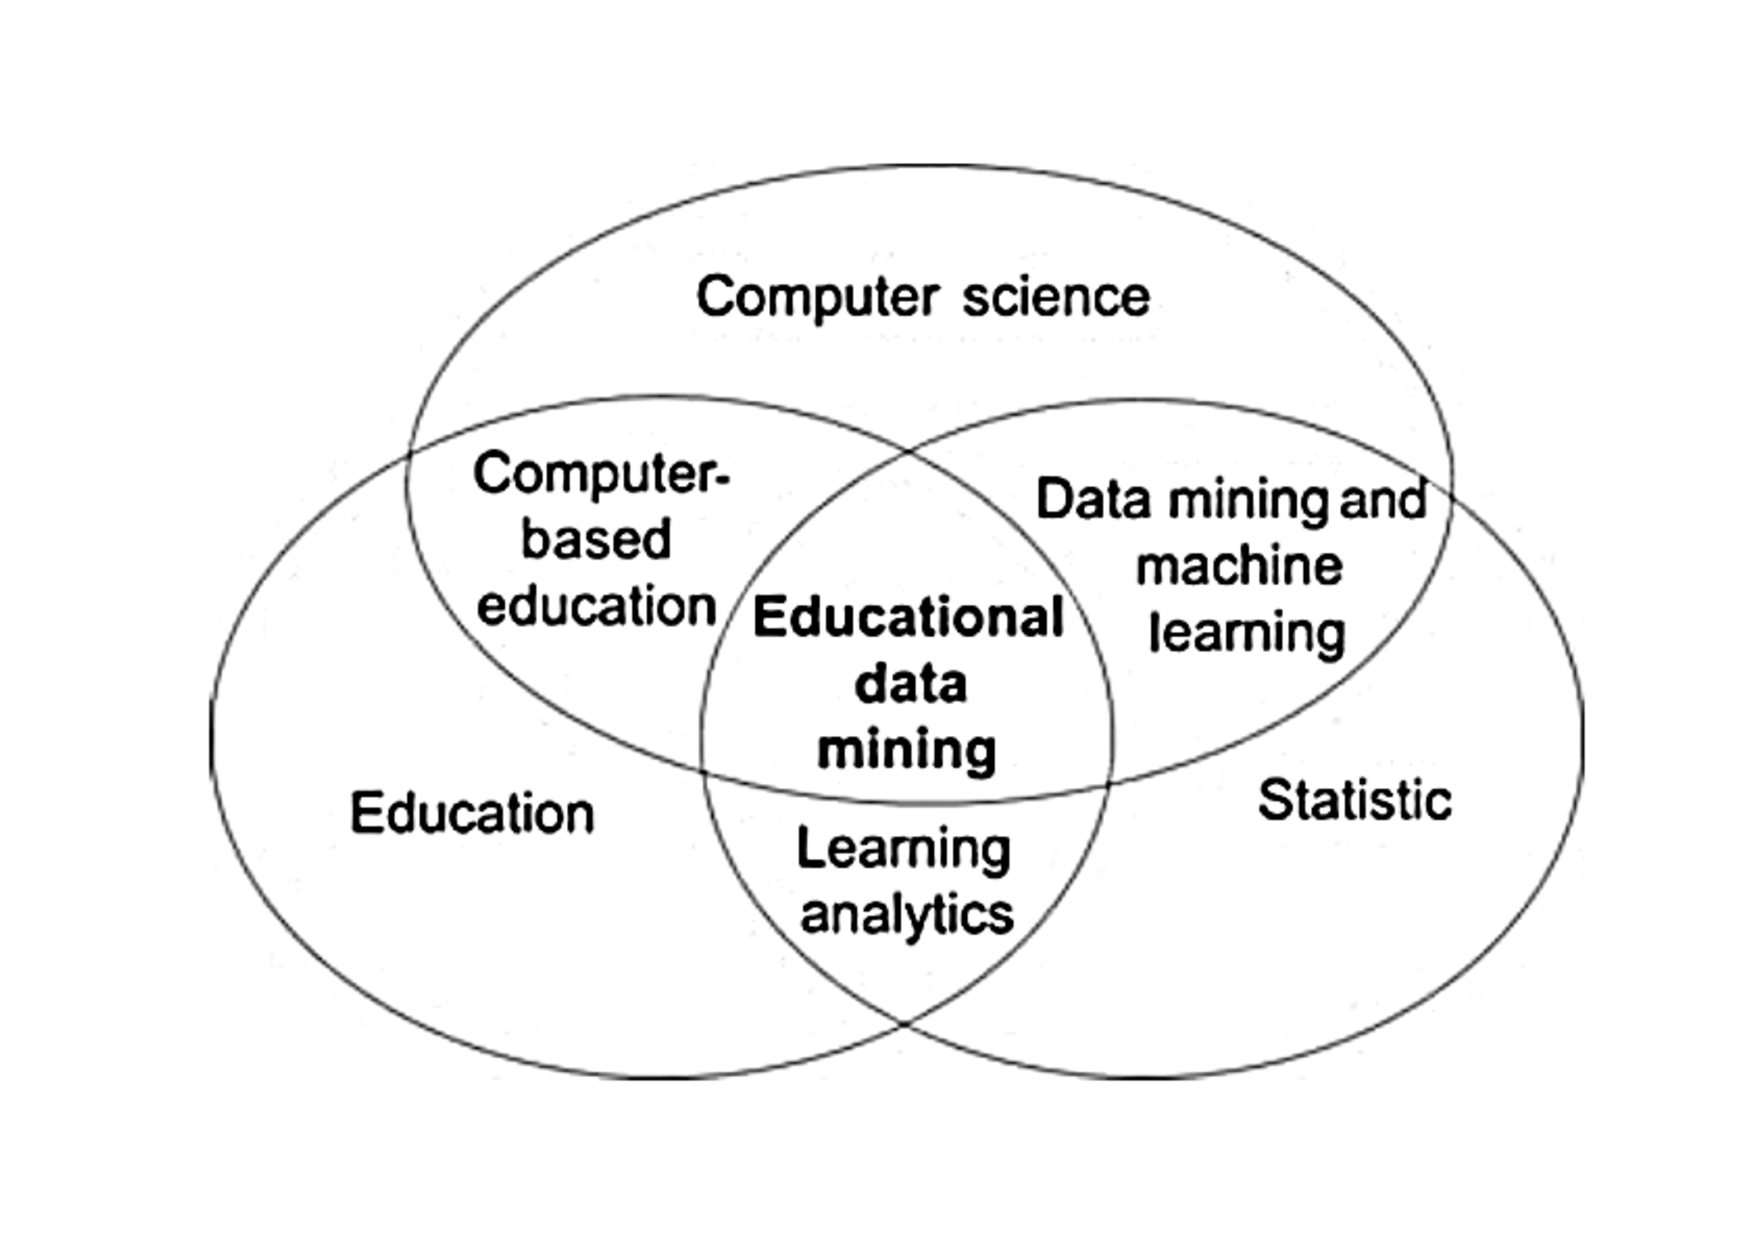
\includegraphics[scale=.4]{imagens/areas-edm.pdf}
  \caption{Principais áreas relacionadas com mineração de dados educacionais. \cite{Koedinger2008}}
  \label{fig:areas-relacionadas-mde}
\end{figure}

%% Predição
% Neste trabalho será aplicado uma tarefa de classificação para tentar resolver o problema de evasão escolar. Segundo \citet{goldschmidt2015data} uma tarefa de classificação possui dois grupos. Um grupo contem normalmente um atributo apenas que vai servir para fazer a predição de um valor (atributo-alvo). Outro grupo corresponde aos atributos que vão servir para fazer a predição do valor (atributos de predição). Tarefas de classificação são largamente utilizadas para fazer a predição de alunos em risco de evasão escolar, como será apresentado mais afrente.

Neste trabalho iremos explorar a utilização de MDE/LA visando classificar e identificar perfis de alunos com tendência a evadir. Segundo \citet{goldschmidt2015data} uma tarefa de classificação possui dois grupos. Um grupo contem normalmente um atributo apenas que vai servir para fazer a predição de um valor (atributo-alvo). Outro grupo corresponde aos atributos que vão servir para fazer a predição do valor (atributos de predição). Tarefas de classificação são largamente utilizadas para fazer a predição de alunos em risco de evasão escolar, como será apresentado nesta proposta.

\citet{baker2010data} agrupa o problema de evasão em uma categoria ou tarefa de detectar o comportamento do aluno. Onde o objetivo é detectar os alunos que têm algum tipo de problema ou comportamento incomum, por exemplo: pouca motivação, trapaça, evasão escolar, etc. Destaca também que as principais técnicas usadas para resolver esses tipos de problemas são de classificação e agrupamentos.

%% 2014
No trabalho de \citet{rigo2014aplicaccoes} é apresentado um estudo de fatores envolvidos no fenômeno de evasão escolar e descrevem a utilização de um sistema para MDE e LA durante 18 meses em cursos de graduação na modalidade de Educação a Distância. Ao todo foram executados 4 experimentos onde foram acompanhados 603, 250, 925 e 713 alunos. Para cada estudo de caso que trata o trabalho foi utilizado a técnica \textit{RNA Multilayer Perceptron}. O melhor resultado com relação a predição da evasão foi no experimento 4 onde a melhor média de acertos foi de 83,7\%.

%% 2015
\citet{pradeep2015students} buscaram prever a evasão de alunos em \textit{middle or secondary education} de uma escola de renome na Índia. O conjunto de dados foi composto por 670 registros de alunos com 57 atributos de estudantes registrados entre 2011 e 2013. Foram usadas 3 fontes de dados diferentes pesquisa com familiares, formulários de admissão e notas dos alunos. O estudo utilizou a ferramenta WEKA: para a seleção de atributos utilizou 7 algoritmos (CfsSubsetEval, ReliefFAttributeEval, ChiSquaredAttributeEval, neRAttributeEval, Consistency-SubsetEval, Filtered AttributeEval, GainRatioAttributeEval) e para a classificação aplicou a técnica de \textit{Decision tree} e \textit{rule induction}. Segundo o autor a qualidade e a confiabilidade das informações disponíveis afetam diretamente os resultados obtidos, por isso é importante reunir as informações corretas. As principais considerações a respeito das técnicas de mineração de dados foram de que os algoritmos se mostraram promissores para fazer a predição de evasão, e a seleção de atributos contribuem para diminuir o número de regras e condições sem perder o desempenho dos classificadores. Com relação ao conhecimento extraído as principais conclusões foram: os métodos de \textit{decision tree} e \textit{induciton rule} são facilmente convertidos em regras \textit{IF-THEM}; alguns atributos que contribuem diretamente para a evasão são notas baixa em matemática, inglês e física, e também alunos com idade acima de 15 anos.

%% 2016
Em \citet{hasbun2016extracurricular} foi discutida a importância de atividades extracurriculares para prever o abandono escolar de estudantes de dois cursos de Bacharel em Ciências (Engenharia e Negócios). Foram coletados dados de 4840 alunos. Dois modelos foram treinados, uma incluindo todos os dados e outra removendo notas e créditos obrigatórios do valor das atividades. Ambos os modelos foram treinados e validados usando \textit{cross-validation}. Utilizou o pacote \textit{R Studio} para o algoritmo CART. A primeira árvore de decisão obteve a melhor precisão (93,94\%). Para o segundo modelo obteve uma precisão de 79,29\%. Os autores relataram que embora a previsão de abandono com dados acumulados mostre um melhor desempenho, o segundo modelo ajuda a resolver o problema de disponibilidade de dados dos alunos. Além disso, a partir da análise dos erros, descobriram que a árvore de decisão treinada com todos os dados foi eficiente na modelagem das expectativas acadêmicas do programa, ocultando fatores pessoais que são mais relevantes para intervenções de prevenção de abandono. Por isso, os resultados apresentados sugerem que incluir atividades extracurriculares é útil para observar comportamentos específicos que parecem estar relacionados ao fenômeno de desligamento relacionado ao abandono.

%% 2017

%% 2018
\citet{lanes2018prediccao} apresentaram um estudo que visa identificar estudantes que apresentam risco de evasão a partir do seu primeiro ano no curso de graduação. Os experimentos foram realizados com informações extraídas do sistema acadêmico da FURG. O conjunto de dados contou com 916 registros de 12 cursos de graduação de áreas distintas. Os dados foram discretizados e categorizados para gerar o \textit{dataset} final. Foi utilizado a ferramenta Weka e aplicado o algoritmo J48 para processar o \textit{dataset} e obter a arvore de decisão. Os resultados mostram que os potenciais alunos em risco de evadir podem ser identificados com acurácia de 90,7\% usando o algoritmo J48.

%% Justificativa

Este trabalho possui como motivação o grande problema de evasão encontrado nos cursos superiores, em especial em alguns cursos sendo principalmente cursos das engenharias e exatas, e a dificuldade de traçar o perfil destes alunos. Além disso, existe uma enorme quantidade de dados históricos de cursos de graduação presencias da UFPEL, uma vez que a grande maioria dos trabalhos vem de cursos EAD. Quanto alguns trabalhos fazem questionários, provas, exercícios, etc, no presente trabalho serão coletado dados que foram gerados a partir de resultado que os alunos obtiveram em diversas disciplinas, cursos entre outros. Este trabalho utilizará a base de dados do Sistema Integrado de Gestão da UFPEL (Cobalto). A base do Cobalto conta também com os dados históricos do GOL que foi o sistema acadêmico da UFPEL de 2006 à 2013. %%

%% Importância acadêmica


%% Distinções entre o trabalho atual e os trabalhos já realizados

\chapter{Objetivos e Resultados}
% (ENTRE 1 e 3 PÁGINAS)

% Este trabalho tem como objetivo estudar e aplicar técnicas de KDD aos dados do sistema Cobalto, para obter um padrão de predição da evasão de alunos através de dados inerentes aos estudantes da UFPEL. Para atingir este objetivo é preciso dividir o trabalho em objetivos específicos.

Este trabalho tem como objetivo estudar e aplicar técnicas de MDE/LA aos dados do sistema Cobalto, para obter um padrão de predição da evasão de alunos através de dados inerentes aos estudantes da UFPEL. Para atingir este objetivo é preciso dividir o trabalho em objetivos específicos.

% O primeiro objetivo específico é investigar o que esta sendo pesquisado na área de mineração de dados educacionais, tentando focar em trabalho que tratam da evasão de alunos.

O primeiro objetivo específico é aprofundar sobre os principais método utilizados em MDE/LA, tentando focar em trabalhos que tratam da evasão escolar. Uma investigação prévia já foi realizada no Trabalho Individual (TI), que focou em encontrar as técnicas mais utilizadas na área de MDE/LA.

Em seguida é preciso fazer um levantamento do referencial teórico e apresentar os principais conceitos a respeito de mineração de dados educacionais. Mais especificamente seria estudar e apresentar os conceitos de KDD, mineração de dados, mineração de dados educacionais, learning analytics. Além disso buscar os principais desafios e oportunidades de aplicação.

Por fim, criar e testar modelos de predição de alunos em risco de evasão de estudantes da UFPEL, utilizando os dados acadêmicos dos alunos. Além de tentar encontrar a melhor forma de apresentar os resultados obtidos.

Em geral a grande maioria dos trabalhos com este foco utilizam base de dados de sistemas de EAD. O grande diferencial deste trabalho é que será utilizado um base de dados histórica consolidada de alunos de graduação da modalidade presencial da UFPEL. Espera-se que os resultados deste trabalho seja aplicado ao sistema acadêmico da UFPEL para ajudar discentes e docentes a prever e combater a evasão.

% Nesta seção, apresentam-se o objetivo Geral e os objetivos Específicos
% da dissertação. Os objetivos não devem ser confundidos com as
% atividades. Para a definição das atividades, deve-se partir dos
% objetivos determinados nesta seção. O objetivo Geral do Projeto
% necessariamente deve ser algum resultado prático (implementação) ou
% teórico (modelos formais ou especificações ou validações) produto da
% pesquisa realizada no período do Projeto. Assim como os objetivos
% específicos, que são considerados como sub-produtos do Objetivo
% Geral. Além disso, deve-se apresentar os principais resultados
% esperados do desenvolvimento desta dissertação.

\chapter{Metodologia}
% (ENTRE 1 e 3 PÁGINAS)

Tomando como ponto de partida os trabalhos encontrados no desenvolvimento do trabalho individual (TI), a dissertação de mestrado seguirá uma metodologia baseada no processo de descoberta de conhecimentos em base de dados (em inglês KDD) e usará a ferramenta de mineração de dados RapidMiner para gerar o conjunto de testes, executar os algoritmos de aprendizagem de máquina e produzir os resultados. Para \citet{fayyad1996kdd} KDD é o processo de descoberta de conhecimento útil de um conjunto de dados, enquanto Mineração de Dados (MD) é apenas parte do processo de KDD. Por isso, considerando o TI como ponto de partida, a elaboração deste trabalho será dividida em 4 etapas: (I) aquisição dos dados, (II) pré-processamento, (III) criar modelos de predição e (IV) avaliar os modelos de predição com base nos modelos de alunos.

Na etapa de aquisição dos dados será separado os dados históricos de alunos do Sistema Cobalto. Este procedimento será feito de forma manual através de consultas na base de dados. Após os dados serão separados e identificados para ser avaliado a qualidade destes dados.

No pré-processamento os dados serão classificados e passarão por um processo de "limpeza" para tentar eliminar ruído dos dados. Esta etapa também será feita de forma manual e é preciso ter um cuidado especial para manter a privacidade dos alunos.

A etapa de gerar o modelo de predição será selecionar, implementar e executar os algoritmos de aprendizagem de máquina. Nesta etapa serão utilizados os algoritmos que obtiveram resultados mais promissores dos artigos selecionados. Além disso, serão gerado modelos de predição para o problema proposto baseado nos dados que foram tratados na etapa anterior.

A ultima etapa os resultados dos experimentos serão avaliados e comparados, para avaliar os conhecimentos extraído. Também será feito um levantamento das principais técnicas usas para avaliar os modelos gerados encontradas nos trabalhos relacionado no TI.

% De forma mais geral a metodologia para elaboração deste trabalho será dividida em 4 etapas: (I)aquisição dos dados, (II)pré-processamento, (III)criar modelos de predição e (IV)avaliar os modelos de predição com base nos modelos de alunos.

% Na etapa de aquisição dos dados será separado os dados históricos de alunos do Sistema Cobalto. Este procedimento será feito de forma manual através de consultas na base de dados. Após os dados serão separados e identificados para ser avaliado a qualidade destes dados.

% No pré-processamento os dados serão classificados e passarão por um processo de "limpeza" para tentar eliminar ruído dos dados. Esta etapa também será feita de forma manual e é preciso ter um cuidado especial para manter a privacidade dos alunos.

% A etapa de gerar o modelo de predição será selecionado, implementado e executado os algoritmos de aprendizagem de máquina. Nesta etapa será utilizado a ferramenta WEKA e serão utilizados os algoritmos que obtiveram resultados mas promissores dos artigos selecionados. Será gerado modelos de predição para o problema proposto baseado nos dados que foram tratados na etapa anterior.
% % A etapa de gerar o modelo de predição será selecionado, implementado e executado os algoritmos de aprendizagem de máquina. Ao final desta etapa serão gerados diversos resultados dos experimentos.

% A ultima etapa os resultados dos experimentos serão avaliados e comparados, para avaliar os conhecimentos extraído.


% Nesta seção, apresenta-se a metodologia proposta para o
% desenvolvimento da Dissertação. O proponente deve descrever as
% atividades necessárias para a conclusão dos objetivos propostos. 

\chapter{Cronograma}

Esta seção apresenta a relação de atividades que deverão ser realizadas e o seu  cronograma para finalização do mestrado em Agosto/2020. As atividades são as seguintes:
\begin{enumerate}
    \item Revisão Bibliográfica: trabalho já realizado e versou sobre descoberta de conhecimento em base de dados;
    \item Aquisição dos Dados: já em andamento consta da extração dos dados do Cobalto;
    \item Pré-processamento: Os dados extraídos do Cobalto passarão por uma limpeza e classificação;
    \item Gerar o modelo de predição: estudar técnicas de mineração de dados aplicadas a educação que mais se adéquam ao problema e aplicar os algoritmos usando o Rapidminer para obter resultados;
    \item Avaliação dos benchmarks dos algoritmos através da ferramenta Rapidminer;
    \item Escrita da  dissertação;
    \item Escrita e submissão de artigo;
    \item Entrega e defensa da dissertação.
\end{enumerate}

\begin{figure}[htbp]
  \centering 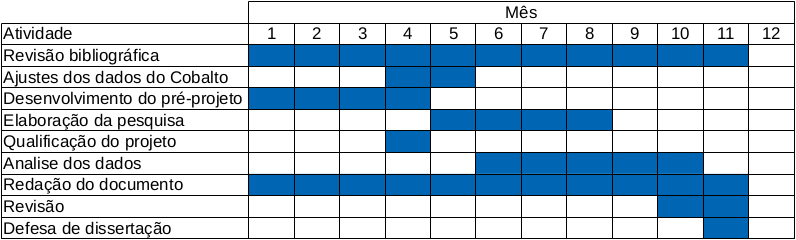
\includegraphics[scale=.4]{imagens/cronograma.png}
  \caption{Cronograma de atividades que serão realizadas.}
  \label{fig:cronograma}
\end{figure}

% Esta seção deve apresentar relação numerada de atividades (de estudo,
% modelagem, especificação, implementação ou validação) que deverão ser
% realizadas (incluindo atividades obrigatórias como seminário de
% andamento, entrega e apresentação da dissertação) e o cronograma
% destas atividades, distribuídas no prazo de 12
% meses.

\bibliography{referencias}
\bibliographystyle{abnt}

\chapter{Assinaturas}
\vspace{2cm}

\begin{center}
\rule{8cm}{.3mm}
\medskip

	Alexandre Gomes da Costa\\
	Proponente

\end{center}

\vspace{4cm}

\begin{center}
\rule{8cm}{.3mm}
\medskip

	Prof. Dr. Julio Carlos Balzano de Mattos\\
	Prof. Orientador

\end{center}

\vspace{4cm}

\begin{center}
\rule{8cm}{.3mm}
\medskip

	Prof. Dr. Tiago Thompsen Primo\\
	Prof. Coorientador

\end{center}
\end{document}
